\documentclass[12pt, twoside]{article}
\usepackage{jmlda}
\usepackage[]{algorithmic}
\usepackage{graphicx}
\usepackage{amsmath}
\usepackage{svg}
\usepackage{multicol}
\usepackage{caption}
\usepackage{subfig}
\newcommand{\hdir}{.}
\graphicspath{{./figures}}
\newtheorem{statement}{Утверждение}

\begin{document}

\title
    []
    {Мультиязычный тематический поиск и категоризация научных публикаций}

\author
    [Е.\,В.~Тищенко]
    {Е.\,В.~Тищенко, К.\,В.~Воронцов}
    [Е.\,В.~Тищенко, К.\,В.~Воронцов, П.\,С.~Потапова]

\abstract{
В статье решается задача кроссязычного поиска текстового плагиата. Целью работы является получение модели, выделяющей информацию о распределении слов в тексте независимо от их языковой принадлежности. Кроме того модель должна удовлетворять ограничениям по размеру и времени обучения для практического использования.

\textbf{Ключевые слова}: \emph{машинное обучение, тематическое моделирование, мультиязыковой поиск дубликатов, обработка текстов на естественном языке, мультиязыковая обработка текстов}
}



\maketitle
\linenumbers
\section{Введение}

Задача поиска и распознавания тематически близких документов является важной из-за невозможности проверить все документы общей тематики на плагиат в силу размеров глобальной сети. Задача становится особенно трудной, так как возникает множество документов, являющихся переводом исходных работ. Согласно исследованиям Donald L. McCabe,\cite{donaldSurvey}  $ 36\% $ студентов американских университетов перефразировали или копировали информацию из всемирной паутины без ссылки на источник. 

Методы векторизации документов для поиска плагиата  \cite{methodMLPlag, regression} преимущественно ограничиваются одним языком. В таком случае возникает проблема создания единообразной системы получения векторных представлений мультиязыковой коллекции документов. Для возможности применения модели за пределами научных экспериментов ставятся технические ограничения ресурсами сервера, а именно на размер модели, временную сложность обучения.

Объектом исследования являются мультиязыковые тематические модели, алгоритмы поиска документов в текстовой коллекции по словам и документам, способы векторного представления слов и документов запроса и коллекции, применяемые для поиска дубликатов независимо от языковой принадлежности.

Тематическая модель коллекции текстовых документов определяет, к каким темам относится каждый документ и какие слова или термины образуют каждую тему. Вероятностная тематическая модель описывает каждую тему дискретным распределением вероятностей слов, а каждый документ $\--$ дискретным распределением вероятностей тем. Тематическая модель преобразует любой текст в вектор вероятностей тем. 

Для решения задачи используется мультимодальная тематическая модель. Такая тематическая модель описывает документы, содержащие метаданные наряду с основым текстом. Под метаданными подразумеваются языковая принадлежность документа, авторство, дата публикации, ссылки на иные источники и многое другое. Метаданные улучшают точность определения тематики документа. В качестве модальностей используются 100 языков, а также научные рубрики Государственного рубрикатора научно-технической информаци ГРНТИ\cite{GRNTI} и Универсального десятичного классификатора УДК\cite{UDK}. Векторное представление текста получается при использовании языков в качестве модальностей. Такое представление независимо от оригинального языка текста. Во время предобработки текста используется BPE токенизация $\--$ итеративная замена наиболее встречаемой пары символов на символ, который не встречается в слове. Этот метод существенно уменьшает объем изначального словаря для практического применения модели.

Целью эксперимента является построение тематической модели для получения векторных представлений текстов. В ходе эксперимента исследуется влияния регуляризации и предобработки текстовых данных на качество поиска. В качестве обучающих данных используются статьи с сайта Wikipedia, а также выборка научных статей из научной электронной библиотеки eLIBRARY.ru.

\section{Постановка задачи поиска дубликатов документов}

Пусть $D~-$ некоторая коллекция документов, $T~-$ множество тем документов. Кандидатом на дубликат  для документа $d \in D$ обозначим такой элемент коллекции $f(d)$, что 

\[f(d) = \argmin_{d' \in D \setminus \{d\}} \rho(m(d), m(d')).\]

В качестве функции $\rho$ используется произвольная метрика векторного пространства. Функция  $m(d) \--$ модель, которая строит векторное представление документа. Качество модели поиска дубликатов измеряется на тестовой выборке при помощи двух метрик сопоставления документов:

1. Средняя частота, с которой документ-запрос попадает в топ 10\%.  Для документа в тестовой выборке уже известно, какие документы являются переводом исходного. Рассматривается доля тех документов, для которых среди 10\% отранжированных кандидатов на дубликат встречаются их переводы. 

2. Средний процент документов в топ 10\% документов-переводов, которые имеют такую же рубрику, что у документа-запроса. Аналогично предыдущей метрике, однако рассматриваются доля тех документов, для которых наиболее близкими в векторном представлении оказываются документы той же рубрики.

Требуется решить задачу поиска дубликатов, при этом качество должно превосходить 0.9 по первой метрке, 0.3 по второй. Также необходимо ограничить размер модели до 100 Гб, а обучение модели должно производиться не более чем за 24 часа.

В качестве преобразования текста в векторном представлении используется тематическое моделирование. Тематическая модель \cite{basetematic}  по коллекции документов строит вероятностное распределение $p(w|t)$ термов w $-$ слов, словосочетаний и терминов в темах $t \in T$. Согласно гипотезе об условной независимости, а также формуле полной вероятности, распределение термов w в документе d является вероятностной смесью распределений термов в темах $\phi_{wt} = p(w|t)$ с весами $\theta_{td}=p(t|d)$:

\[p(w|d) = \sum_{t \in T} p(w|t, d)p(t|d) = \sum_{t \in T} p(w|t)p(t|d) =\sum_{t\in T}\phi_{wt}\theta_{td}.\]

Данное выражение можно переписать в матричном виде. Матрица частот термов в документах

\[F \approx \Phi \Theta.\]

Так как число тем, как правило, намного больше, чем число документов, то требуется найти такое разложение, ранг которого не превосходит $|T|$.


\section{Вычислительный эксперимент}

Cтавится задача поиска оптимальных параметров тематической модели, методов токенизации текста, при которых будут достигнуты требования на качество модели и удовлетворены физические ограничения. После выбора оптимальных параметров будут проведены эксперименты, показывающие вклад каждого отдельного решения на общее качество модели.

Тестовая выборка генерируется определенным образом. Поиск тематически близкого документа производится не по всей поисковой коллекции, а по подвыборке документов, в которой 10\% документов имеет такую же рубрику УДК, что и документ-запрос, а остальные 90\% документов имеют другую рубрику УДК.

В качестве метрики в векторном пространстве используется метрика аналогий. Пусть $A$ ~--- язык ориганального докумена $d$, а поиск производится среди документов $d'$ на языке $B$. Тогда 

\[\rho(d, d') = 1 - cos(d', d - a + b)\]
где $a$ и $b$ ~--- средние вектора по всем документам коллекции, принадлежащим языкам $A$ и $B$ соответственно.

\subsection{Описание данных}

Для обучения тематической модели использовались статьи научной электронной библиотеки eLibrary\cite{eLib}, а также многоязычной интернет-энциклопедии Wikipedia\cite{wiki}. %, описанные в работе \cite{}. % Как сослаться на статью, которую ещё не опубликовали?. 
Для подавляющего числа научных статей eLibrary были известны рубрики ГРНТИ и УДК. Формирование выборки статьей на 100 языках происходило следующим образом. Было отобрано 24 тысячи статей библиотеки eLibrary на русском и английском языках. Затем статьи были переведены на 42 языка. Языки были выбраны по причине их большой представленности среди научных текстов. Перевод осуществлялся при помощи системы статистического машинного перевода Moses \cite{Moses}. Также для всех языков, включая эти 42, были собраны статьи из энциклопедии Wikipedia.

Ниже представлено распределение обучающих данных по рубрикам УДК и ГРНТИ. Стоит отметить несбалансированность выборок по объему документов, что влечет проблемы при обучении, так как предполагается обучать модель на сбалансированных данных. Кроме того среди рубрик ГРНТИ присутствует рубрика <<нет>>, которая представляет набор документов, не принадлежащих к другим рубрикам. Данная рубрика содержит документы, относящиеся к различным темам и является четвертой по размеру среди всех рубрик.

\begin{figure}[H]
  \subfloat{\includesvg[width=0.5\textwidth]{udc_ru.svg}}
  \subfloat{\includesvg[width=0.5\textwidth]{grnti_ru.svg}}
 \caption{Распределение данных по рубрикам УДК и ГРНТИ}
  \label{fig:1}
\end{figure}

\subsection{Базовые модели}

В качестве базовой модели используется тематическая модель, использующая в качестве модальностей 100 языков, см. Табл. 3. Обучение происходит на основе данных Википедии. Используются 300 тем, из них одна является фоновой. Фоновая тема содержит все общеупотребимые слова, не являющиеся предметными. К ним относятся предлоги, частицы, союзы и другие неинформативные части речи. При предобработке текста используется метод BPE токенизации, причем изначальный объем словаря в 120 тысяч токенов ужат до 2 тысяч для каждого отдельного языка. Обучение модели занимает порядка 6 часов, а размер модели составляет 4.6 Гб. 

В качестве альтернативной базовой модели рассматривается нейросетевая модель XLM-RoBERTa\cite{Roberta}. Данная модель обучена на 2.5TB данных, содержащих документы на 100 различных языках. Векторное представление текста получается путем усреднения ембеддингов отдельных предложений. Получение векторного представения отдельного текста занимает в среднем 1.6 секунды, однако из-за большого размера коллекции документов общее время получения эмбеддингов занимает 120 часов.

\section{Предложенное решение}

Применение к базовой тематической модели различных эвристик, а также поиск оптимальных параметров позволяет добиться требуемых результатов. Ниже представлен список принятых решений для повышения качества модели:

\begin{enumerate}

\item При обучении модели подбирается оптимальное количество тем в промежутке от 10 до 1000. Наилучшие результаты были достигнуты при выделении 125 отдельных тем. Существенный прирост вносит добавление модальностей рубрик УДК и ГРНТИ. 

\item Обучение тематической модели происходит итеративно, на каждой итерции отбирается случайная подвыборка документов. Для решения проблемы несбалансированности данных относительно рубрик, на каждой итерации обучения генерируется подвыборка документов, для которой распределение рубрик ГРНТИ оказалось равномерным. Таким образом, в каждой подвыборке документов количество документов с различными рубриками одинаково.

\item Уменьшение словаря до 2 тыс. токенов на язык позволяет учесть ограничения на размер модели, однако такого количества токенов недостаточно для описания отдельного языка. Использование 11 тыс. токенов позволяет не только улучшить выразительность модели, а значит ее качество, но и соблюдать ограничения на время обучения, которое составляет не более 24 часов.

\item Использование рубрики <<нет>> снижает качество модели, так как в ней представлены документы различной тематики. Для повышения качества модели принято решение не учитывать эту рубрику и не устанавливать ее в качестве модальности для документов. Помимо этого решено исключить стоп-слова из 15 основных языков.

\end{enumerate}

Обучение занимает 25 итераций, на рис. 2 представлено, как изменяются метрики в зависимости от номера итерации.

% \begin{figure}[h]
% \centering
%   \subfloat{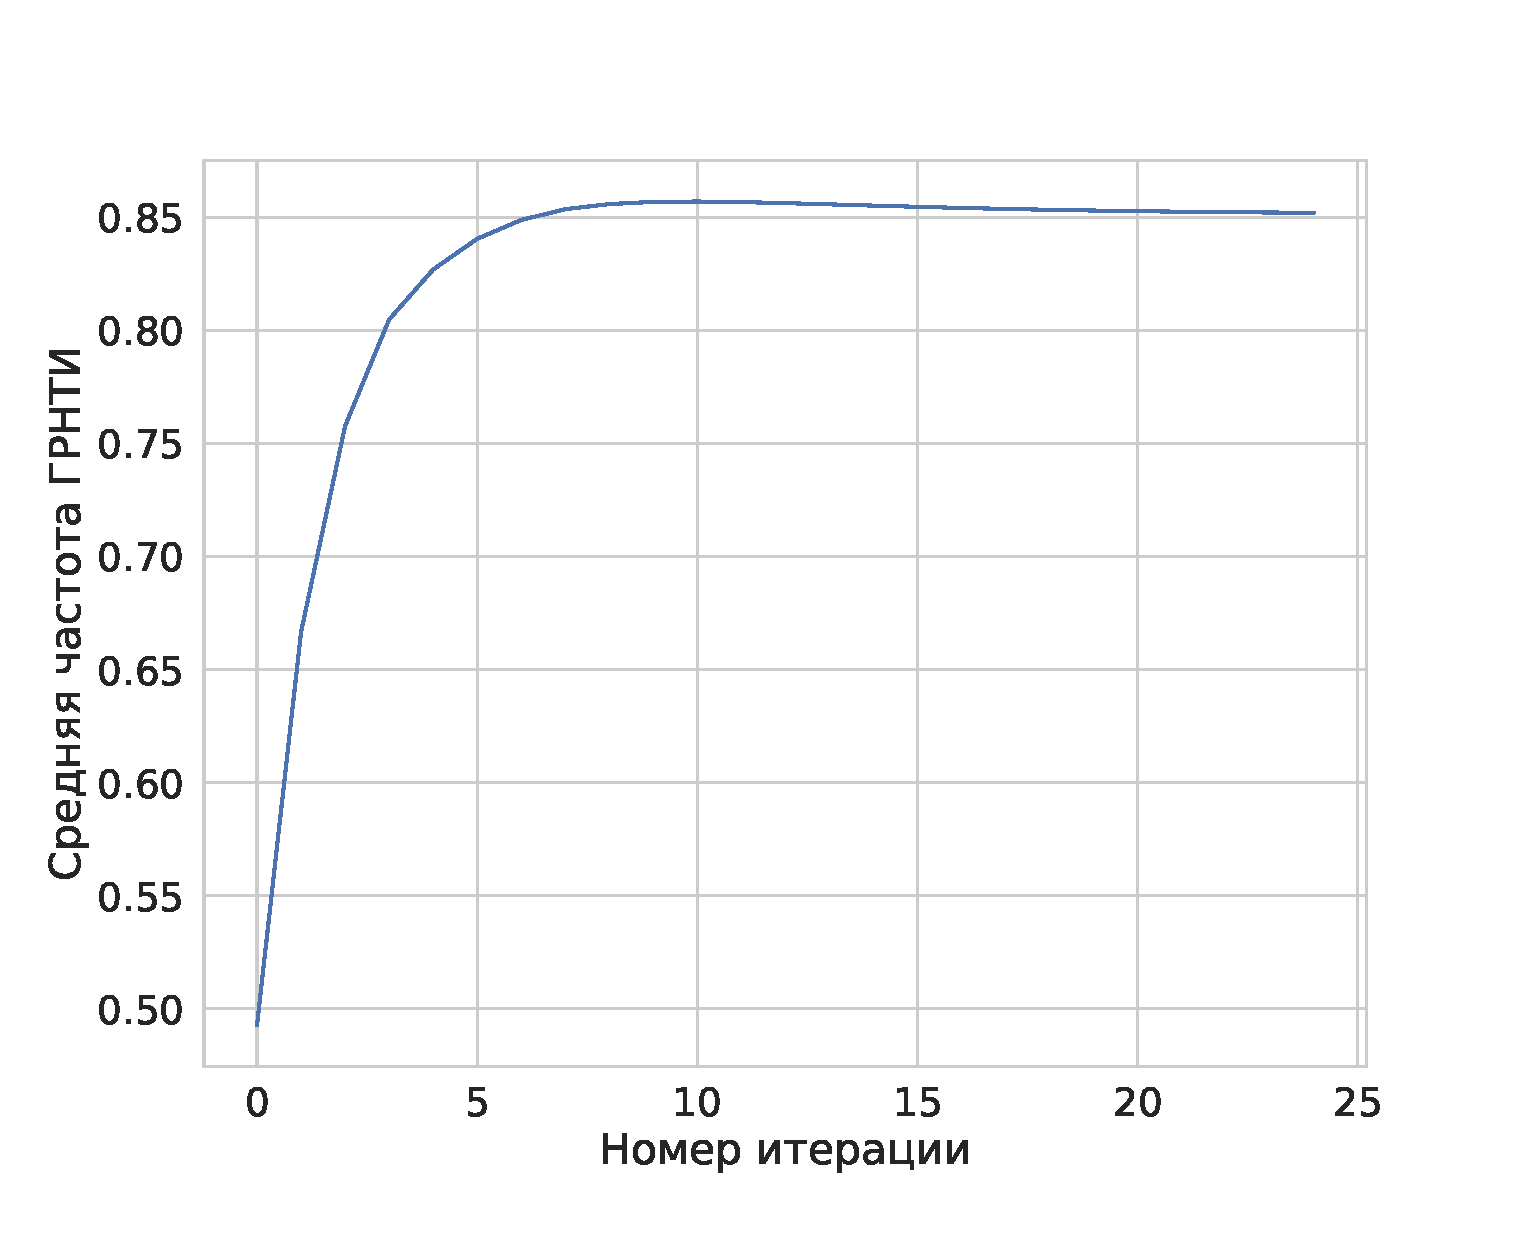
\includegraphics[width=0.5\textwidth]{error.eps}}
%  \caption{Средняя частота ГРНТИ в зависимотси от итерации обучения}
%   \label{fig:1}
% \end{figure}

\begin{figure}[H]
  \subfloat{\includesvg[width=0.5\textwidth]{res_freq_ru.svg}}
  \subfloat{\includesvg[width=0.5\textwidth]{res_perc_ru.svg}}
 \caption{Качество модели во время обучения}
  \label{fig:1}
\end{figure}

\subsection{Результаты экспериментов}

Ниже представлено сравнение базовых решений с итоговым.

\begin{table}[h]
\caption {Сравнение моделей} \label{tab:title} 
\centering
\begin{tabular}{|l|c|c|c|c|}
\hline
\multicolumn{1}{|l|}{Название модели} & \begin{tabular}[c]{@{}c@{}}Средняя\\ частота\\ УДК\end{tabular} & \begin{tabular}[c]{@{}c@{}}Средний\\ процент\\ УДК\end{tabular} & \begin{tabular}[c]{@{}c@{}}Средняя\\ частота\\ ГРНТИ\end{tabular} & \begin{tabular}[c]{@{}c@{}}Средний\\ процент\\ ГРНТИ\end{tabular} \\ \hline
Базовая тематическая модель           & 0.558                                                           & 0.165                                                           & 0.536                                                             & 0.220                                                             \\ \hline
XLM-RoBERTa                           & 0.835                                                           & 0.179                                                           & 0.832                                                             & 0.288                                                             \\ \hline
Итоговая тематическая модель          & \textbf{0.995}                                                  & \textbf{0.225}                                                  & \textbf{0.852}                                                    & \textbf{0.366}                                                    \\ \hline
\end{tabular}
\end{table}

Как видно из таблицы, качество итоговой тематической модели сильно отличается от базового решения, а также от модели XLM-RoBERTa. По всем метрикам итоговая модель показала лучшее качество.

В таблице 3 указано качество тематической модели, которая была обучена без определенного признака. Как можно заметить, наибольший вклад в качество модели внесло решение о расширении словаря до 11 тыс. токенов.


\begin{table}[h]
\centering
\caption {Сравнение важности признаков} \label{tab:title} 
\begin{tabular}{|l|c|c|c|c|}
\hline
Название модели  & \begin{tabular}[c]{@{}c@{}}Средняя\\ частота\\ УДК\end{tabular} & \begin{tabular}[c]{@{}c@{}}Средний\\ процент\\ УДК\end{tabular} & \begin{tabular}[c]{@{}c@{}}Средняя\\ частота\\ ГРНТИ\end{tabular} & \begin{tabular}[c]{@{}c@{}}Средний\\ процент\\ ГРНТИ\end{tabular} \\ \hline
Итоговая тематическая модель                                                              & \textbf{0.995}                                                  & \textbf{0.225}                                                  & \textbf{0.852}                                                    & \textbf{0.366}                                                    \\ \hline
Использование 300 тем вместо 125                                                          & 0.714                                                           & 0.185                                                           & 0.663                                                             & 0.232                                                             \\ \hline
Использование 11 тыс. токенов вместо 2 тыс.                                               & 0.539                                                           & 0.163                                                           & 0.499                                                             & 0.195                                                             \\ \hline
\begin{tabular}[c]{@{}l@{}}Генерация выборок с одинаковым \\ количеством тем\end{tabular} & 0.834                                                           & 0.197                                                           & 0.789                                                             & 0.262                                                             \\ \hline
\end{tabular}
\end{table}



\section{Заключение}

В данной работе предложен метод получения векторного представления текста с использованием тематического моделирования, позволяющего получать по документу вектор вероятностей принадлежности отдельным темам независимо от их языковой принадлежности.

Были рассмотрены базовая тематическая модель, а также нейросетевая модель XLM-RoBERTa. Обе модели были протестированы на коллекции документов, принадлежащих 42 различным языкам.

Были предложены различные эвристики, а также метод предобработки текста, улучшающий качество тематической модели, при этом были соблюдены ограничения на размер модели и время обучения для практического использования. Проведено сравение итоговой тематической модели с базовыми.

\begin{thebibliography}{8}

\bibitem{donaldSurvey}
    \BibAuthor{Donald L. McCabe}
    Cheating among college and university students: A North American perspective//
    \BibJournal{International Journal for Educational Integrity}, 2005
    
\bibitem{methodMLPlag}
    \BibAuthor{Zdenek Ceska, Michal Toman, and Karel Jezek}
    Multilingual Plagiarism Detection//
    \BibJournal{Artificial Intelligence: Methodology, Systems and Applications}, 2008
    
\bibitem{regression}
    \BibAuthor{Duygu Ataman, Jose G. C. de Souza, Marco Turchi, Matteo Negri}
    Cross-lingual Semantic Similarity Measurement Using Quality Estimation Features and Compositional Bilingual Word Embeddings//
    

\bibitem{GRNTI}
  \textit{grnti.ru}
  
\bibitem{UDK}
  \textit{udcsummary.info}
    
\bibitem{basetematic}
    \BibAuthor{Воронцов К. В.}
    Обзор вероятностных тематических моделей.//
    
\bibitem{eLib}
  \textit{elibrary.ru}   
  
\bibitem{wiki}
  \textit{wikipedia.org}
  
\bibitem{Moses}
  \textit{Koehn P. et al.} Moses: Open source toolkit for statistical machine translation //Proceedings of the 45th annual meeting of the association for computational linguistics companion volume proceedings of the demo and poster sessions. – 2007. – С. 177-180.

\bibitem{Roberta}
  \textit{Alexis Conneau, Kartikay Khandelwal, Naman Goyal, Vishrav Chaudhary, Guillaume Wenzek, Francisco Guzmán, Edouard Grave, Myle Ott, Luke Zettlemoyer, Veselin Stoyanov} Unsupervised Cross-lingual Representation Learning at Scale.
	  
\end{thebibliography}

\section{Аппендикс}
В таблице представлены все языки, на основе которых происходило обучение тематической модели.

\begin{table}[H]
\caption {Представленные языки} \label{tab:title} 
\begin{tabular}{|l|l|l|l|l|l|l|l|}
\hline
1  & Английский    & 26 & Арабский         & 51 & Узбекский     & 76 & Бирманский           \\ \hline
2  & Немецкий      & 27 & Персидский       & 52 & Интерлингва   & 77 & Каракалпакский       \\ \hline
3  & Французский   & 28 & Финский          & 53 & Галисийский   & 78 & Амхарский            \\ \hline
4  & Русский       & 29 & Сербо-хорватский & 54 & Малаялам      & 79 & Сомали               \\ \hline
5  & Испанский     & 30 & Сербский         & 55 & Албанский     & 80 & Самоа                \\ \hline
6  & Итальянский   & 31 & Словенский       & 56 & Валлийский    & 81 & Гуджарати            \\ \hline
7  & Португальский & 32 & Иврит            & 57 & Боснийский    & 82 & Лаосский             \\ \hline
8  & Китайский     & 33 & Африкаанс        & 58 & Бенгальский   & 83 & Идиш                 \\ \hline
9  & Японский      & 34 & Литовский        & 59 & Таджикский    & 84 & Кирунди              \\ \hline
10 & Чешский       & 35 & Индонезийский    & 60 & Непальский    & 85 & Яванский             \\ \hline
11 & Польский      & 36 & Греческий        & 61 & Суахили       & 86 & Ромашнский           \\ \hline
12 & Турецкий      & 37 & Хинди            & 62 & Туркменский   & 87 & Татарский            \\ \hline
13 & Датский       & 38 & Тайский          & 63 & Молдавский    & 88 & Чеченский            \\ \hline
14 & Казахский     & 39 & Каталонский      & 64 & Эсперанто     & 89 & Башкирский           \\ \hline
15 & Киргизский    & 40 & Малайский        & 65 & Гаэльский     & 90 & Чувашский            \\ \hline
16 & Корейский     & 41 & Белорусский      & 66 & Сингальский   & 91 & Аварский             \\ \hline
17 & Шведский      & 42 & Эстонский        & 67 & Монгольский   & 92 & Кабардино-черкесский \\ \hline
18 & Венгерский    & 43 & Исландский       & 68 & Язык басков   & 93 & Ингушский            \\ \hline
19 & Нидерландский & 44 & Азербайджанский  & 69 & Малагасийский & 94 & Осетинский           \\ \hline
20 & Румынский     & 45 & Латвийский       & 70 & Тамильский    & 95 & Якутский             \\ \hline
21 & Норвежский    & 46 & Латинский        & 71 & Кхмерский     & 96 & Карачаево-балкарский \\ \hline
22 & Болгарский    & 47 & Грузинский       & 72 & Урду          & 97 & Лезгинский           \\ \hline
23 & Хорватский    & 48 & Македонский      & 73 & Маори         & 98 & Эрзянский            \\ \hline
24 & Украинский    & 49 & Армянский        & 74 & Алеутский     & 99 & Марийский            \\ \hline
\end{tabular}
\end{table}

\end{document}
